\documentclass[12pt,fleqn]{article}
\linespread{2}

	\addtolength{\oddsidemargin}{-.875in}
	\addtolength{\evensidemargin}{-.875in}
	\addtolength{\textwidth}{1.75in}

	\addtolength{\topmargin}{-.875in}
	\addtolength{\textheight}{1.75in}

\usepackage[round, comma, authoryear, sort]{natbib}
\bibliographystyle{agufull04}

\newcommand{\beginsupplement}{%
        \setcounter{table}{0}
        \renewcommand{\thetable}{S\arabic{table}}%
        \setcounter{figure}{0}
        \renewcommand{\thefigure}{S\arabic{figure}}%
     }
\usepackage{setspace}
\usepackage{caption} 
\captionsetup[figure]{font={footnotesize,stretch=1}}
\captionsetup[table]{font={footnotesize,stretch=1}}

\usepackage{lineno}


%% MATH

\usepackage{latexsym, amsmath, amscd,amsthm,amssymb}
\newcommand{\tand}{\text{ and }}
\newcommand{\tfor}{\text{ for }}
\newcommand{\twith}{\text{ with }}
\newcommand{\twhere}{\text{ where }}
\newcommand{\ton}{\text{ on }}
\newcommand{\tin}{\text{ in }}
\newcommand{\tif}{\text{ if }}
\newcommand{\tor}{\text{ or }}
\newcommand{\tis}{\text{ is }}


\usepackage{graphicx}

\usepackage{fancyvrb}
\usepackage{relsize}
\DefineVerbatimEnvironment{VerbIn}{Verbatim}{fontsize=\relsize{-1}}
\DefineVerbatimEnvironment{VerbOut}{Verbatim}{fontshape=it,fontsize=\relsize{-1}}




\begin{document}


\author{Betsy Cowdery}
\title{}
\date{December 12, 2014}

\maketitle


\begin{abstract}

Developing large-scale quantification of leaf trait relationships are key to building robust terrestrial ecosystem models. However, current plant trait data is limited by space and scope. The  goal of this project is to develop a multivariate Bayesian meta-analytical model that synthesizes necessary plant trait data from multiple studies while accounting for various sources of uncertainty. Using observed sample mean, sample size, and a sample error statistics for multiple plant traits, we aim to produced well constrained estimates of mean and precision for a single trait. This has been done using a univariate model, however, a multivariate model can leverage the fact that many plant traits are highly correlated to constrain our estimates even further.  

\end{abstract}


\newpage
\linenumbers
\section{Introduction}

Developing large-scale quantification of leaf trait relationships are key to building robust terrestrial ecosystem models. Although there exist many of plant trait datasets, observations are not evenly distributed across the world. Areas that easily accessible and have economically important species of plants will produce the largest datasets. Similarly, some plant characteristics are more difficult to measure than others and will be studied less frequently. By quantifying the relationships between plant traits, we can use the data we have to predict the values that we lack \citep{Wright,Reich2007}. 

In 2004 \citep{Wright} found that six plant traits (leaf mass per area, leaf lifespan, leaf nitrogen per unit mass, photosynthetic capacity per unit leaf mass, leaf dark respiration rate per unit mass  and leaf phosphorus concentration per unit mass), independent of classifications such as ‘plant functional types’ (PFTs), are all highly correlated. In fact, almost three-quarters of the global variation in these six traits was captured by a simple regression model through six-dimensional space \citep{Wright2005}. The next step is to build more complex models to increase our predictive power. 

In this study I will implement simple univariate and multivariate Bayesian meta-analytical models to the same data used in these previous studies. Bayesian meta-analysis allows us to combine plant trait data from across numerous studies, leveraging the strong correlations between the plant traits, one can produce better constrained estimates of mean and precision for a each plant trait \citep{Dietze2014} . Furthermore, Bayesian models can be designed to accommodate data with missing values, thus increasing our sample size and strengthening our predictive power \citep{Clark2007}.

\section{Materials and Methods}

\subsection{Experimental Data}
the data used in this project is compiled from the global plant trait network (GLOPNET), a database created to quantify leaf economics across the world’s plant species. The total database consists of 2548 species–site combinations from 175 sites. There are 2021 different species in total, with 342 species occurring at more than one site. These data are described in detail and are available as supplemental material in \citep{Wright}. 

In the dataset there are six plant-traits provided: leaf mass per area (LMA), leaf lifespan (LL), leaf nitrogen per unit mass (Nmass), photosynthetic capacity per unit leaf mass (Amass), leaf dark respiration rate per unit mass (Rmass) and leaf phosphorus concentration per unit mass (Pmass). Each variable has been log transformed. 

\subsection{Bayesian Models}

Following \citep{LEBAUER2013}, I assume that the sample mean for each plant trait is drawn from a normal distribution. In the univariate case, the means are drawn individually, but in the multivariate case they are drawn simultaneously. The prior distributions for each plant trait are set to be uninformative. 

\noindent First let $Y_{i,j}$ be the $j$th observation of the $i$th trait.

\noindent{\bf Univariate Model}\\
\begin{linenomath*}
$Y_{i,j} \sim N(\mu_{i,j}, \sigma^2)$ (Data model)\\
$\sigma^2 \sim IG(s_1,s_2)$ (Error variance prior) \\
$\mu_{i,j} \sim N(\mu_0, V_\mu)$ (Fixed effects prior)
\end{linenomath*}\\
The model was translated into BUGS (Bayesian inference Using Gibbs Sampling) code through JAGS (Just another Gibbs Sampler). \citep{Gelman2013, Leb2013, LEBAUER2013, Lebauer2013, Plummer2010} 

\begin{singlespace}
\begin{VerbIn}
model{
  prec.sigma~dgamma(.001,.001) # uninformative prior on precision (1/variance)
  sigma <- 1/prec.sigma
  for(i in 1:n){mu[i]~dnorm(0,.001)} # uninformative prior for fixed effects
  
  for(i in 1:N){
      for(j in 1:n){
          Y[i,j]~dnorm(mu[j],prec.sigma)
          }
      }
  }
\end{VerbIn}
\end{singlespace}

\noindent In the multivariate model, $Y_{i,j}$ becomes a latent variable, and $Y^{(0)}_{i,j}$ is the observed value.  \\
\noindent{\bf Multivariate Model}\\
$Y_i \sim N_p(\vec{\mu}_i, \Sigma) $ (Process Model)\\
$Y^{(0)}_{i,j} \sim N_p(Y_{i,j}, \tau^2)$ (Data Model)\\
$\tau^2 \sim IG(t_1,t_2)$ (Observation error prior) \\ 
$\mu_{i,j} \sim N(\mu_0, V_\mu)$ (Fixed effects prior)\\
$\Sigma \sim IW(V, df)$ (Process error prior)  \begin{singlespace}
 \begin{VerbIn}
model{
  prec.Sigma~dwish(Vsig[,],n)  # uninformative prior on precision
  Sigma[1:n,1:n] <- inverse(prec.Sigma[,])
  
  mu[1:n]~dmnorm(mu0[],Vmu)    # uninformative prior for fixed effects
  
  for(i in 1:N){
      Y[i,1:n]~dmnorm(mu[],prec.Sigma[,])
      for(j in 1:n){
          X[i,j]~dnorm(Y[i,j],10000000) # observation error is set to very low  
          }
      }
  }
 \end{VerbIn}
\end{singlespace}

\noindent Each of the models was run with the full GLOPNET dataset and with a subset of the dataset in which all studies with missing observations were excluded. 


\section{Results and Discussion}

Figure 1 provides a visual summary of the GLOPNET dataset. Each of the two plot matrices in figure 1 consist of three parts. The lower left half of the plot matrix shows scatterplots of each combination of variables with  a fit lowess curve in red. The top right half of the plot matrix shows pairwise correlation. The plots on the diagonal show histograms of the collected data. The lefthand matrix shows all the available data and the righthand matrix shows only studies in which every plant trait was measured. This significantly reduces the sample size from 2548 to 72. 

When looking at the full dataset, every plant trait has a statistically significant correlation with all the others, which suggests that a multivariate analysis will in fact be informative. Using the limited dataset, correlation values are lower and one pair of traits no longer have a statistically significant correlation. It is clear from this summary why we need models that accommodate data with missing values. 

Figure 2 shows plots of the posterior distributions for each plant trait after running the univariate and multivariate models for the full and subsetted datasets. When using data that excludes studies with missing observations, there appears to be practically no difference between the two model’s estimated means for each of the variables. However, for both models, including studies with NA’s produces estimated means that are clearly different from those produced with data excluding NA’s. For the variables Log.LMA and Log.Amass, the estimated means from the univariate and multivariate models were very close, but for the remaining variables, they were noticeably different, with the estimated mean from the univariate model always closer to the data mean than the estimated mean from the multivariate model.

Contrary to what one might expect, the variation in the multivariate model showed little to no improvement over the univariate.  The multivariate model produced posterior distributions with larger variance around the mean (except for Log.Nmass where the SE for the univariate model was larger by 3.3e-06, a small amount relative to the size of the mean.) When studies with missing observations are included, the standard errors show signs of improvement. The posterior distributions from the multivariate model have smaller variances for all the variables except Log.Pmass. However, it is difficult to see the difference since the expected means of the variables are no longer similar.

The shapes of the individual plant trait posteriors make more sense when we look at them alongside joint distributions with other variables. Figure 3 shows one such combination. The other fourteen join density distributions are displayed in Supplemental figure 3. In figure 3, the four 95\% confidence ellipses of the joint density distributions for Log.LMA and Log.Amass corresponding with the four model runs. Plotted inside each ellipse is the normalized eigenvectors of the covariance matrix. Along the x and y axes are plotted the corresponding probability density functions found in figure 2 (not to scale, merely for reference). In this plot we can see that the effect of adding in studies with missing observations has a dramatic impact on the area of the confidence region. For both the univariate and multivariate case, including NA's decreases the area of the confidence region. Introducing the multivariate model also changed the shape and sizes of the joint probability confidence regions. However, the changes can be subtle and it's east to see how these changes do not translate back into the single trait probability density curves. This turns out to simply be the ratio of the square roots of the eigenvalues of the covariance matrix. 

In an effort to quantify the differences in ellipse shapes, I calculated the ratio of the lengths of the major and minor axes of each ellipse.
$$ r= \frac{2 \sqrt{\lambda_1}\sqrt{\frac{p(n-1)}{n(n-p)}F_{p,n-p}(\alpha)}}{2 \sqrt{\lambda_2}\sqrt{\frac{p(n-1)}{n(n-p)}F_{p,n-p}(\alpha)}} = \frac{ \sqrt{\lambda_1}}{ \sqrt{\lambda_2}}$$
where $(\lambda_1, \lambda_2 )$ are the eigenvectors of the covariance matrix between the two traits being compared, $n$ is the sample size, $p=2$ is degrees of freedom and level of significance $\alpha = .05$ \citep{Johnson2007}. Table S1 contains of results for each of the fifteen pairs. In almost every case the multivariate model produced more elongated confidence ellipses. The four exceptions were joint distributions of Log.Rmass with Log.LL, Log.LMA, Log.Amass, and Log.Pmass.

\section{Conclusion}

Applying Bayesian models to the GLOPNET data has proven to be useful in two very important ways: first of all our Bayesian models(both univariate and multivariate) can handle data with missing values. This changed the sample size from 72 to 2548. Such a considerable increase in sample size helped to constrain parameter estimates. Second, introducing a multivariate model, changed the shape and sizes of the joint probability confidence regions. The changes at times were subtle and could go undetected when projected back into single probability functions. However, changes such as decreased overall area and increases in elongation of the confidence ellipse will improve our estimation of plant traits. These models have shown an overall improvement in our ability to predict plant trait. However, they are nowhere near complete. There are many opportunities for adding in additional complexity such as random effects for site as well as informing specific plant trait priors. 

\newpage
\begin{singlespace}
\bibliography{/Users/elizabethcowdery/Documents/Bib/GE509_Project.bib}
\end{singlespace}

\newpage
\section{Figures and Tables}

\begin{figure}[h]
  \makebox[\textwidth][c]{
    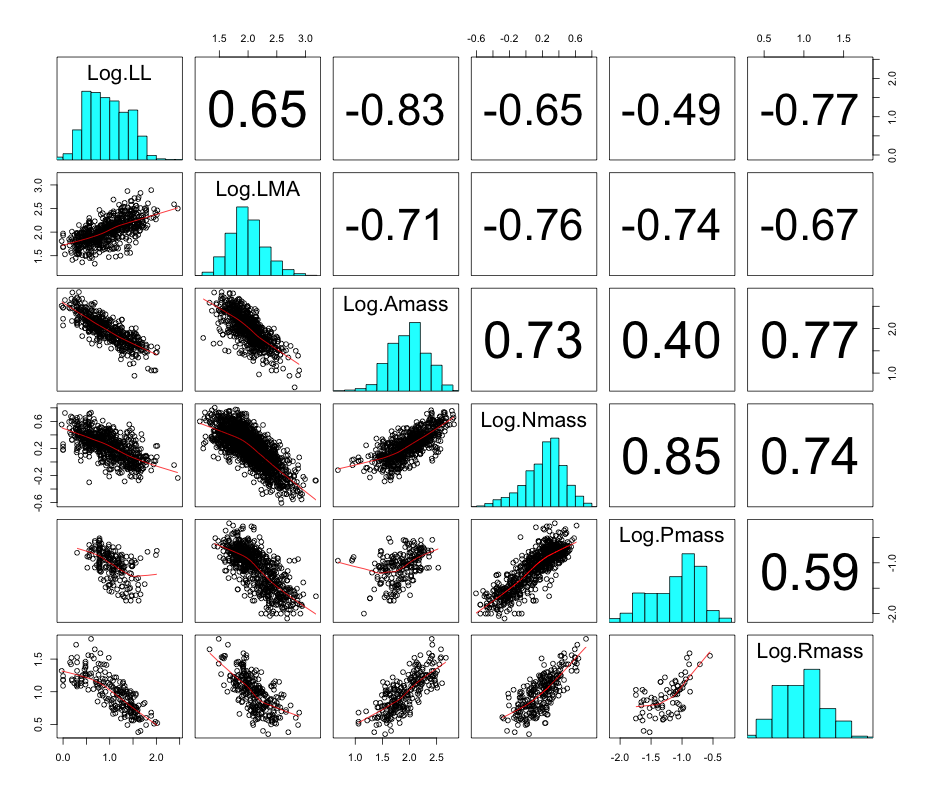
\includegraphics[width=.55\textwidth]{corr_na.png}
    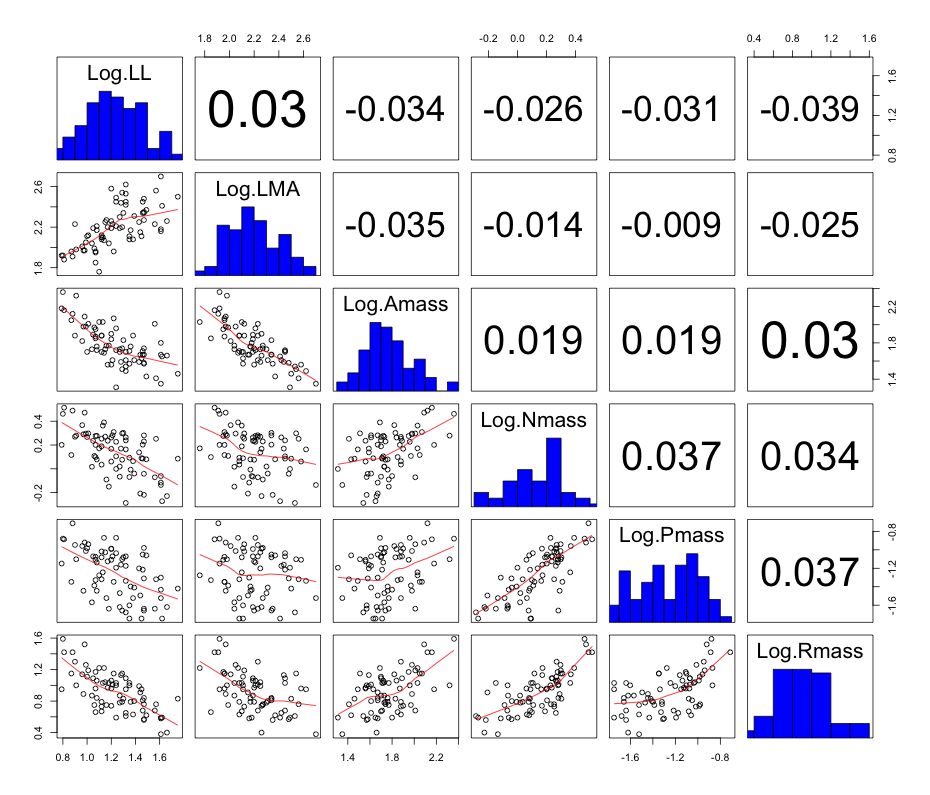
\includegraphics[width=.55\textwidth]{corr.png}}%
  \caption{Visual summary of the GLOPNET dataset. The lower left half of the plot matrices show scatterplots of each combination of variables with a fit lowess curve in red. The top right half of the plot matrices show pairwise correlation values. The plots on the diagonals show histograms of the collected data. The lefthand matrix shows statistics for all the available data and the righthand matrix shows statistics excluding observations with missing values}
  \label{fig:key}
\end{figure}


\begin{figure}[h]
  \makebox[\textwidth][c]{
    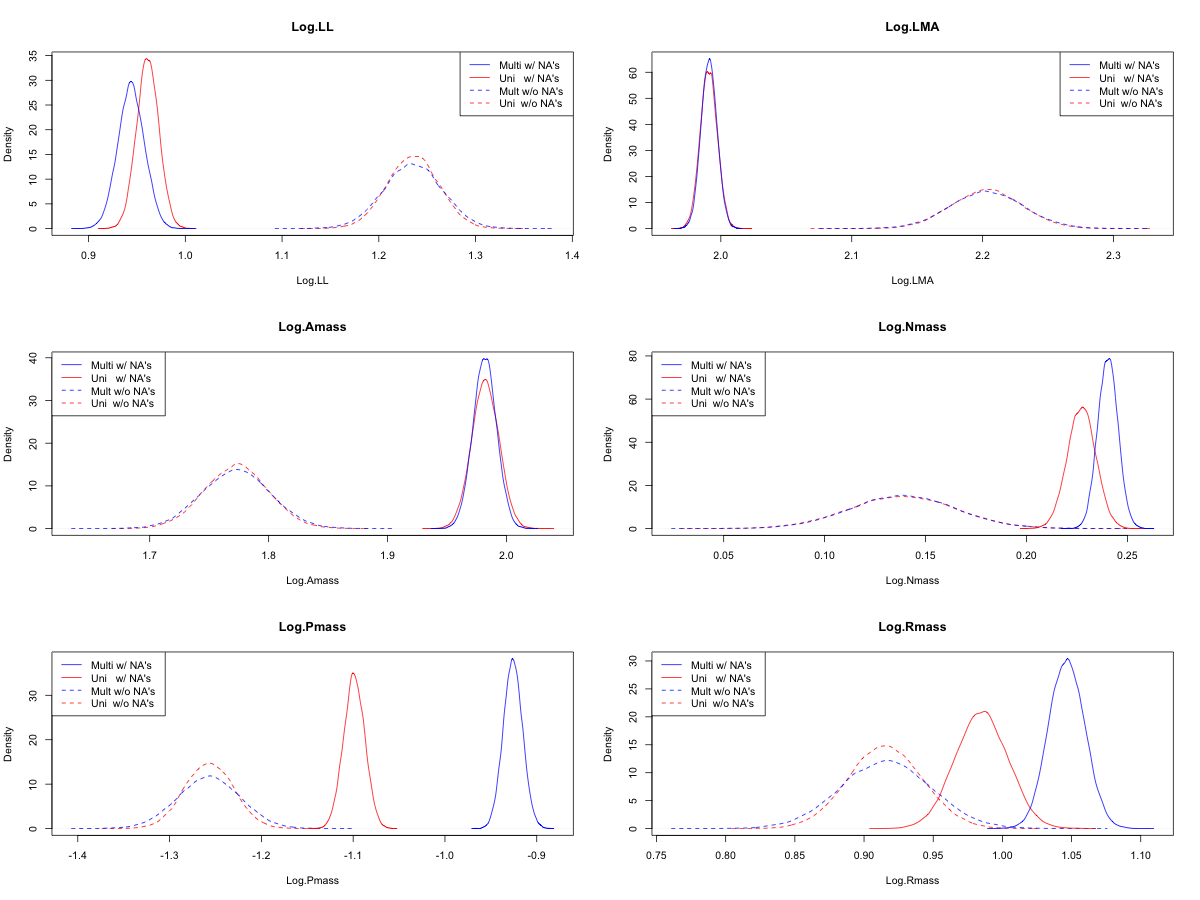
\includegraphics[width=1\textwidth]{dist.png}}%
  \caption{Posterior distributions for each plant trait after running the four model runs : univariate without NA's (red dashed), univariate with NA's (red solid), multivariate without NA's (blue dashed), multivariate with NA's (blue solid).}
  \label{fig:key}
\end{figure}

\begin{figure}[h]
  \makebox[\textwidth][c]{
    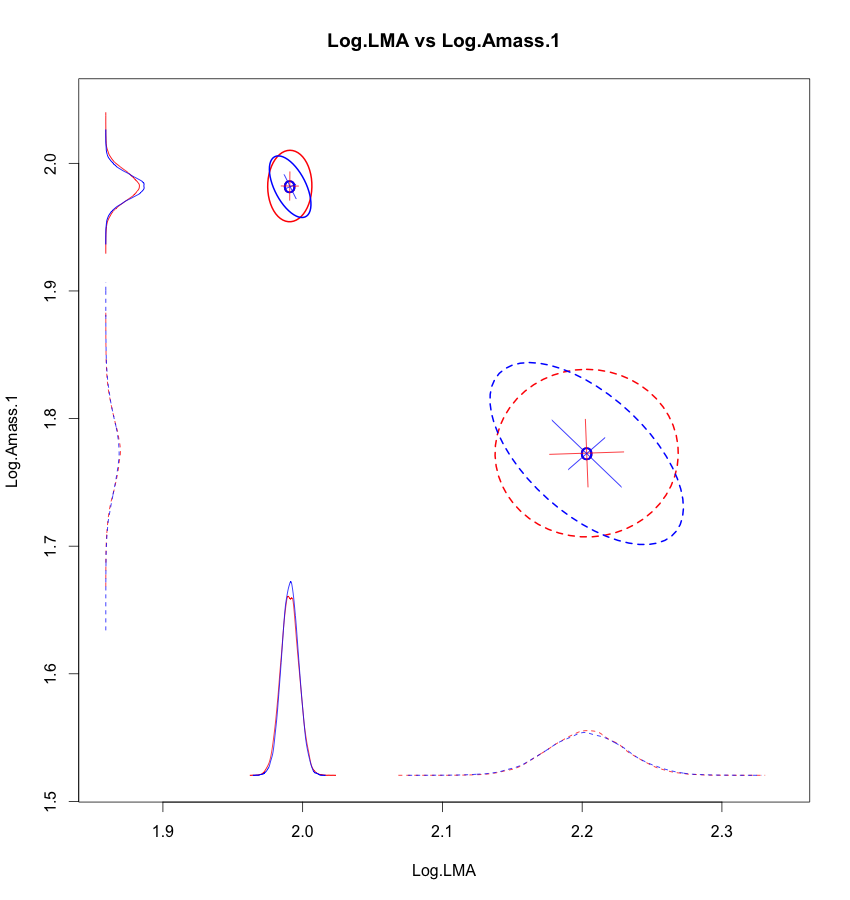
\includegraphics[width=.55\textwidth]{joint_dist.png}}%
  \caption{Joint density 95\% confidence ellipses for the pairs of plant traits Log.LMA and Log.Amass for four model runs : univariate without NA's (red dashed), univariate with NA's (red solid), multivariate without NA's (blue dashed), multivariate with NA's (blue solid). Plotted inside each ellipse is the normalized eigenvectors of the covariance matrix. Along the x and y axes are plotted the corresponding probability density functions found in figure 2}
  \label{fig:key}
\end{figure}

\newpage
\newpage 
\section {Supplementary Figures and Tables}
\beginsupplement

\begin{table}[hb]
\centering
\caption{Ratios of the lengths of the major and minor axes of each joint density 95\% confidence ellipse}
\begin{tabular}{rrrrr}
  \hline
   & Univariate & Multivariate & Univariate & Multivariate \\ 
 & excluding NA & excluding NA & including NA & including NA \\ 
  \hline
Log.LL vs Log.LMA & 1.00 & 1.73 & 1.78 & 2.73 \\ 
  Log.LL vs Log.Amass & 1.01 & 1.80 & 1.01 & 2.39 \\ 
  Log.LL vs Log.Nmass & 1.01 & 1.68 & 1.65 & 3.36 \\ 
  Log.LL vs Log.Pmass & 1.01 & 1.58 & 1.00 & 1.62 \\ 
  Log.LL vs Log.Rmass & 1.00 & 1.88 & 1.65 & 1.45 \\ 
  Log.LMA vs Log.Amass & 1.00 & 1.98 & 1.77 & 2.28 \\ 
  Log.LMA vs Log.Nmass & 1.01 & 1.32 & 1.08 & 2.43 \\ 
  Log.LMA vs Log.Pmass & 1.01 & 1.26 & 1.78 & 2.15 \\ 
  Log.LMA vs Log.Rmass & 1.01 & 1.53 & 2.93 & 2.33 \\ 
  Log.Amass vs Log.Nmass & 1.01 & 1.48 & 1.64 & 2.67 \\ 
  Log.Amass vs Log.Pmass & 1.01 & 1.37 & 1.01 & 1.50 \\ 
  Log.Amass vs Log.Rmass & 1.01 & 1.60 & 1.66 & 1.62 \\ 
  Log.Nmass vs Log.Pmass & 1.00 & 2.07 & 1.65 & 2.85 \\ 
  Log.Nmass vs Log.Rmass & 1.01 & 1.96 & 2.72 & 2.87 \\ 
  Log.Pmass vs Log.Rmass & 1.01 & 1.64 & 1.65 & 1.37 \\ 
   \hline
\end{tabular}
\end{table}

\begin{table}[ht]
\centering
\caption{Correlation matrix for the six plant traits in the GLOPNET database, excluding observations with missing values}

\begin{tabular}{rrrrrrr}
  \hline
 & Log.LL & Log.LMA & Log.Amass & Log.Nmass & Log.Pmass & Log.Rmass \\ 
  \hline
Log.LL & 0.0512 & 0.0301 & -0.0335 & -0.0255 & -0.0310 & -0.0392 \\ 
  Log.LMA & 0.0301 & 0.0422 & -0.0345 & -0.0138 & -0.0090 & -0.0249 \\ 
  Log.Amass & -0.0335 & -0.0345 & 0.0468 & 0.0195 & 0.0191 & 0.0297 \\ 
  Log.Nmass & -0.0255 & -0.0138 & 0.0195 & 0.0342 & 0.0372 & 0.0339 \\ 
  Log.Pmass & -0.0310 & -0.0090 & 0.0191 & 0.0372 & 0.0690 & 0.0368 \\ 
  Log.Rmass & -0.0392 & -0.0249 & 0.0297 & 0.0339 & 0.0368 & 0.0637 \\ 
   \hline\end{tabular}
\end{table}

\begin{table}[ht]
\centering
\caption{Posterior correlation matrix from the multivariate model for the six plant traits in the GLOPNET database, excluding observations with missing values}

\begin{tabular}{rrrrrrr}
  \hline
 & Log.LL & Log.LMA & Log.Amass & Log.Nmass & Log.Pmass & Log.Rmass \\ 
  \hline
Log.LL & 0.0661 & 0.0305 & -0.0340 & -0.0258 & -0.0315 & -0.0397 \\ 
  Log.LMA & 0.0305 & 0.0571 & -0.0350 & -0.0140 & -0.0091 & -0.0252 \\ 
  Log.Amass & -0.0340 & -0.0350 & 0.0618 & 0.0198 & 0.0194 & 0.0302 \\ 
  Log.Nmass & -0.0258 & -0.0140 & 0.0198 & 0.0489 & 0.0377 & 0.0343 \\ 
  Log.Pmass & -0.0315 & -0.0091 & 0.0194 & 0.0377 & 0.0843 & 0.0372 \\ 
  Log.Rmass & -0.0397 & -0.0252 & 0.0302 & 0.0343 & 0.0372 & 0.0789 \\ 
   \hline
\end{tabular}
\end{table}


\begin{table}[ht]
\centering
\caption{Posterior correlation matrix from the multivariate model for the six plant traits in the GLOPNET database, including observations with missing values}
\begin{tabular}{rrrrrrr}
  \hline
 & Log.LL & Log.LMA & Log.Amass & Log.Nmass & Log.Pmass & Log.Rmass \\ 
  \hline
Log.LL & 0.2481 & 0.1052 & -0.1625 & -0.0855 & -0.1272 & -0.1221 \\ 
  Log.LMA & 0.1052 & 0.0902 & -0.0860 & -0.0524 & -0.0747 & -0.0655 \\ 
  Log.Amass & -0.1625 & -0.0860 & 0.1445 & 0.0688 & 0.0955 & 0.0941 \\ 
  Log.Nmass & -0.0855 & -0.0524 & 0.0688 & 0.0558 & 0.0701 & 0.0573 \\ 
  Log.Pmass & -0.1272 & -0.0747 & 0.0955 & 0.0701 & 0.1329 & 0.0790 \\ 
  Log.Rmass & -0.1221 & -0.0655 & 0.0941 & 0.0573 & 0.0790 & 0.0977 \\ 
   \hline
\end{tabular}
\end{table}

\begin{figure}[h]
  \makebox[\textwidth][c]{
    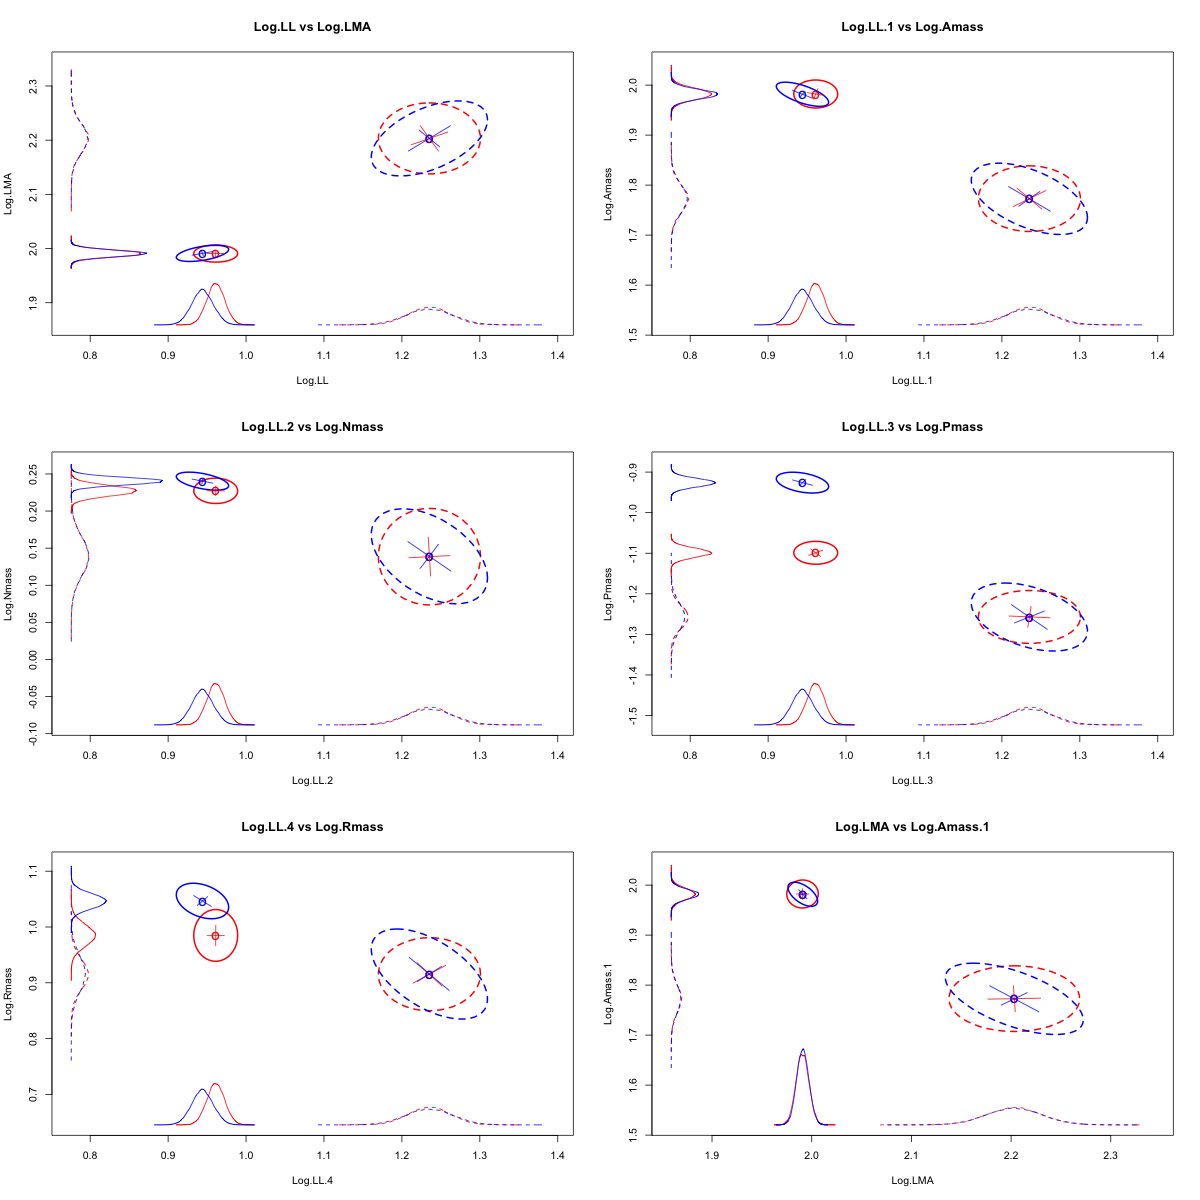
\includegraphics[width=1\textwidth]{P1.png}}%
  \caption{Joint density 95\% confidence ellipses for pairs of plant traits corresponding with the four model runs : univariate without NA's (red dashed), univariate with NA's (red solid), multivariate without NA's (blue dashed), multivariate with NA's (blue solid). Plotted inside each ellipse is the normalized eigenvectors of the covariance matrix. Along the x and y axes are plotted the corresponding probability density functions found in figure 2}
  \label{fig:key}
\end{figure}
\begin{figure}[h]
  \makebox[\textwidth][c]{
    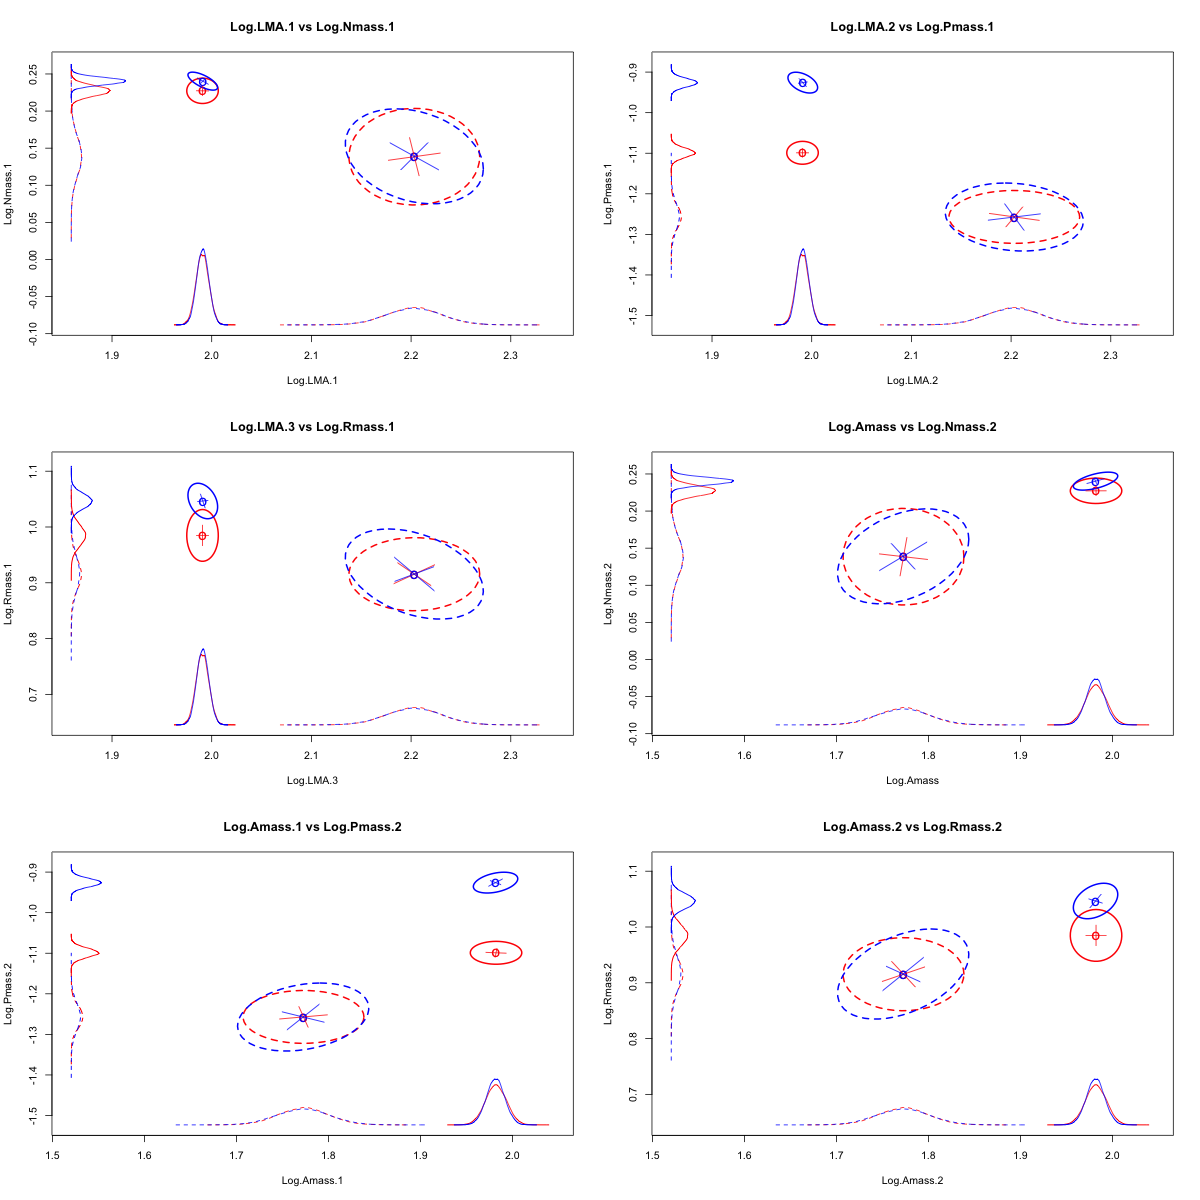
\includegraphics[width=1\textwidth]{P2.png}}%
  \caption{Joint density 95\% confidence ellipses for pairs of plant traits corresponding with the four model runs : univariate without NA's (red dashed), univariate with NA's (red solid), multivariate without NA's (blue dashed), multivariate with NA's (blue solid). Plotted inside each ellipse is the normalized eigenvectors of the covariance matrix. Along the x and y axes are plotted the corresponding probability density functions found in figure 2}  \label{fig:key}
\end{figure}
\begin{figure}[h]
  \makebox[\textwidth][c]{
    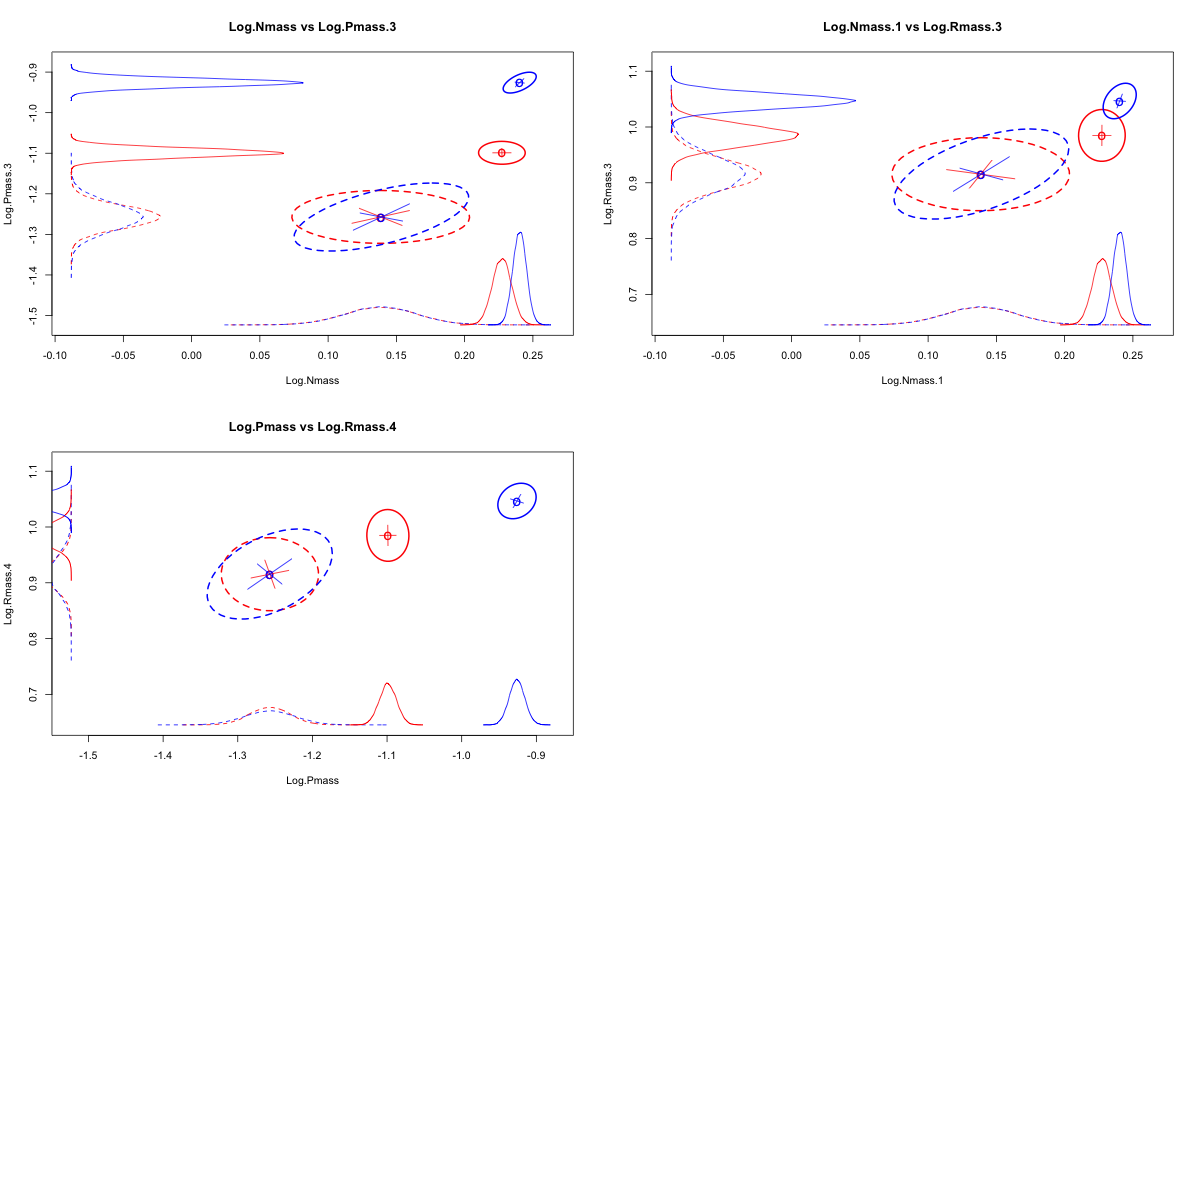
\includegraphics[width=1\textwidth]{P3.png}}%
  \caption{Joint density 95\% confidence ellipses for pairs of plant traits corresponding with the four model runs : univariate without NA's (red dashed), univariate with NA's (red solid), multivariate without NA's (blue dashed), multivariate with NA's (blue solid). Plotted inside each ellipse is the normalized eigenvectors of the covariance matrix. Along the x and y axes are plotted the corresponding probability density functions found in figure 2}
  \label{fig:key}
\end{figure}


\end{document}